\documentclass[xcolor=svgnames, 10pt, aspectratio=169]{beamer}

% packages 
\usepackage{graphicx}
\usepackage{tikz}
\usepackage{lmodern}
\usepackage{booktabs}
\usepackage{multirow}
\usepackage{tabularx}
\usepackage{natbib}
\usepackage{bibentry}
\usepackage{tcolorbox}
\usepackage{caption}
\usepackage{setspace}
\usepackage{adjustbox}
\usepackage{listings}
\usepackage{parcolumns}
\usepackage{textcomp} 
\usepackage{algorithm}
\usepackage{algpseudocode}

\lstset{ %
language=Matlab,
numbers=none,           % where to put the line-numbers
numberstyle=\tiny,      % the size of the fonts that are used for the line-numbers
basicstyle=\footnotesize,    % the size of the fonts that are used for the line-numbers
escapeinside={(*@}{@*)}
}

% don't display Figure or Table before caption
\captionsetup[figure]{labelformat=empty}% redefines the caption setup of the figures environment in the beamer class.

% Algorithms
\renewcommand{\thealgorithm}{2.\arabic{algorithm}}
\setcounter{algorithm}{0}

% space, not comma between author and year
\setcitestyle{aysep={}}

% Fonts
\usepackage{mathpazo}

% Template Setup
\setbeamertemplate{frametitle}{\vskip+3pt \insertframetitle \vskip+3pt \usebeamerfont{framesubtitle}\usebeamercolor[fg]{framesubtitle}\insertframesubtitle \vskip-1pt \noindent \centerline{\rule{\textwidth}{0.4pt}}}
\setbeamerfont{frametitle}{series=\bfseries, size=\Large}
\setbeamerfont{framesubtitle}{series=\bfseries, size=\normalsize}
\setbeamercolor{frametitle}{fg=myblue}
\setbeamercolor{framesubtitle}{fg=black}
\setbeamercolor{title}{fg=myblue}
\setbeamercolor{date}{fg=myblue}

% Colors
\colorlet{myblue}{MidnightBlue!60!black!82}
\colorlet{myred}{Red!60!black!82}

% tikz 
\usepackage{tikz}
\usetikzlibrary{spy,calc,arrows,decorations.pathreplacing}

% Set up the `tcolorboxes'
\tcbset{
    noparskip,
    colback=Silver!8, 
    colframe=myblue, 
    boxrule=0.3pt,
    coltext=black,
    coltitle=white, 
    fonttitle=\large\bfseries
    }
    
% Links
\setbeamercolor{button}{bg=myblue,fg=white}    

% Itemize Item
\setbeamercolor{itemize item}{fg=myblue, bg=white}
\setbeamercolor{itemize subitem}{fg=myblue, bg=white}
\setbeamercolor{itemize subsubitem}{fg=myblue, bg=white}

\setbeamertemplate{itemize item}{\Large \raise-1pt \hbox{\textbullet}} 
\setbeamertemplate{itemize subitem}{\large \raise-1pt \hbox{\textbullet}} 
\setbeamertemplate{itemize subsubitem}{\small \raise-1pt \hbox{\textbullet}} 

% Remove navigation bar
\beamertemplatenavigationsymbolsempty

% Include frame number
%\setbeamertemplate{footline}[frame number]

% start full screen
%\hypersetup{pdfpagemode=FullScreen}

% At the beginning of every section
\AtBeginSection[]
{
  \begin{frame}
    \vfill 
    \centering
    {\color{myblue} \bfseries \huge \insertsectionhead}
    \vfill 
 
  \end{frame}
}

% Macros


% Statistics
\newcommand\pN{\mathcal{N}} % Normal distribution
\newcommand\iidN{\overset{iid}{\sim}\mathcal{N}} % iid Normal
\newcommand\E{\mathbb{E}} % Expectations Operator
\newcommand\transpose[1]{{#1}^{\sf{T}}}

% Title Page
\title{ \bfseries \LARGE Precision-based sampling with missing observations}
\date{\vfill \bfseries Kiel Institute Research Seminar \\[4pt] March 22\textsuperscript{nd}, 2022}	

\author[shortname]{
                   Philipp Hauber\inst{1,2}
                }  

\institute[shortinst]{
                      \inst{1} JMU Würzburg \\
                      \inst{2} Kiel Institute for the World Economy (IfW)                        
                     }
 
% Body of the presentation
\begin{document}

%\setbeamertemplate{footline}{} % don't display slide numbers!
\begin{frame}
	\vskip+5.5pt
    \centerline{\rule{1.1\textwidth}{0.4pt}}
	
    \maketitle

    \centerline{\rule{1.1\textwidth}{0.4pt}}
\end{frame}   

\begin{frame}{This presentation}{}
    Mash-up of two papers in my dissertation!\\~\\

    

    Method: 
    \vspace{0.1cm}

    Hauber, P and C. Schumacher (2021). \textit{Precision-based sampling with missing observations: A factor model application}, \textbf{Bundesbank Discussion Paper 11/2021}.
    \\~\\
    Application:  
    \vspace{0.1cm}

    Hauber, P. (2021) \textit{How useful is external information from professional forecasters? Conditional forecasts in large factor models} \medskip
\end{frame}

\begin{frame}{Motivation}

Essential task in the Bayesian estimation of state space models: drawing from $p(\boldsymbol{\eta} | \mathbf{y}, \Theta)$ where $\boldsymbol{\eta}$ is an unobserved component, $\mathbf{y}$ is data and $\Theta$ parameters \\~\\

Precision-based samplers (\citealp[][\scriptsize \textbf{IJMMNO}\normalsize]{chanjelizakov_2009}; \citealp[][\scriptsize \textbf{JEcmtrics}\normalsize]{mccausland_2012}) exploit the fact the precision matrix of $\boldsymbol{\eta}$ is banded in many macroeconomic application $\rightarrow$ alternative to simulation smoothers that rely on the Kalman filter \\~\\

Applications in macroeconomics (with complete data) include models of trend inflation (\citealp[][\scriptsize \textbf{JBES}\normalsize]{chankooppotter_jae2013}), time-varying Bayesian vector autoregressions \citep[][\scriptsize \textbf{JBES}\normalsize]{chan_2020jbes} and factor models (\citealp[][\scriptsize \textbf{JAE}\normalsize]{kaufmannschumacher_jae2017})\\~\\

Missing observations arise frequently in macroeconomic applications/datasets: different starting dates, different release patterns ("ragged edge"), outliers or mixed frequencies\\~\\

In our paper, we propose a precision-sampler that can handle (most of these) applications! 

\end{frame}

\begin{frame}{Precision-based sampling}{Simple example}
AR(2) process: $\eta_t = \phi_1 \eta_{t-1} + \phi_2 \eta_{t-2} + u_t; \, u_t \sim \mathcal{N}(0, \sigma^2)$ \\~\\

Stacking the observations over $t = 1, \dots, T$ yields 
$$
\mathbf{H} \boldsymbol{\eta} = \mathbf{u}, \: \text{where} \: \mathbf{u} \sim \mathcal{N}(0, \mathbf{I}_T \sigma^2) \: \text{and} \:
\mathbf{H} = 
\left[
\begin{smallmatrix}
1 &  &  &  &  \\
-\phi_1 & 1 &  &  &  \\
-\phi_2 & -\phi_1 & 1 &  &  \\
 & -\phi_2 & -\phi_1 & 1 &  &  \\
 &  & \ddots & \ddots & \ddots &  & \\
 &  &  &  -\phi_2 & -\phi_1 & 1
\end{smallmatrix}
\right]
$$ \medskip


$\boldsymbol{\eta}$ is Normal with mean $\mathbf{0}_T$ and covariance matrix $\Sigma = \mathbf{H}^{-1} \, \mathbf{I}_T\sigma^{2} \, \transpose{\mathbf{H}^{-1}}$ \\~\\

corresponding \textit{precision matrix} is given by $\mathbf{Q} = \Sigma^{-1} = \transpose{\mathbf{H}} \, \mathbf{I}_T\sigma^{-2} \, \mathbf{H}$
\end{frame}

\begin{frame}{Precision-based sampling with missing observations}{Covariance and precision matrix of $\boldsymbol{\eta}$}

    Properties of the multivariate $\mathcal{N}$: 

    \begin{itemize}
        \item $\Sigma_{ij} = 0$ $\Longrightarrow$ independence of $\eta_i$ and $\eta_j$
        \item $\mathbf{Q}_{ij} = 0$ $\Longrightarrow$ \textbf{conditional} independence of $\eta_i$ and $\eta_j$ \\~\\
    \end{itemize}    

    \begin{adjustbox}{minipage=0.7\textwidth,center}
        \begin{figure}
            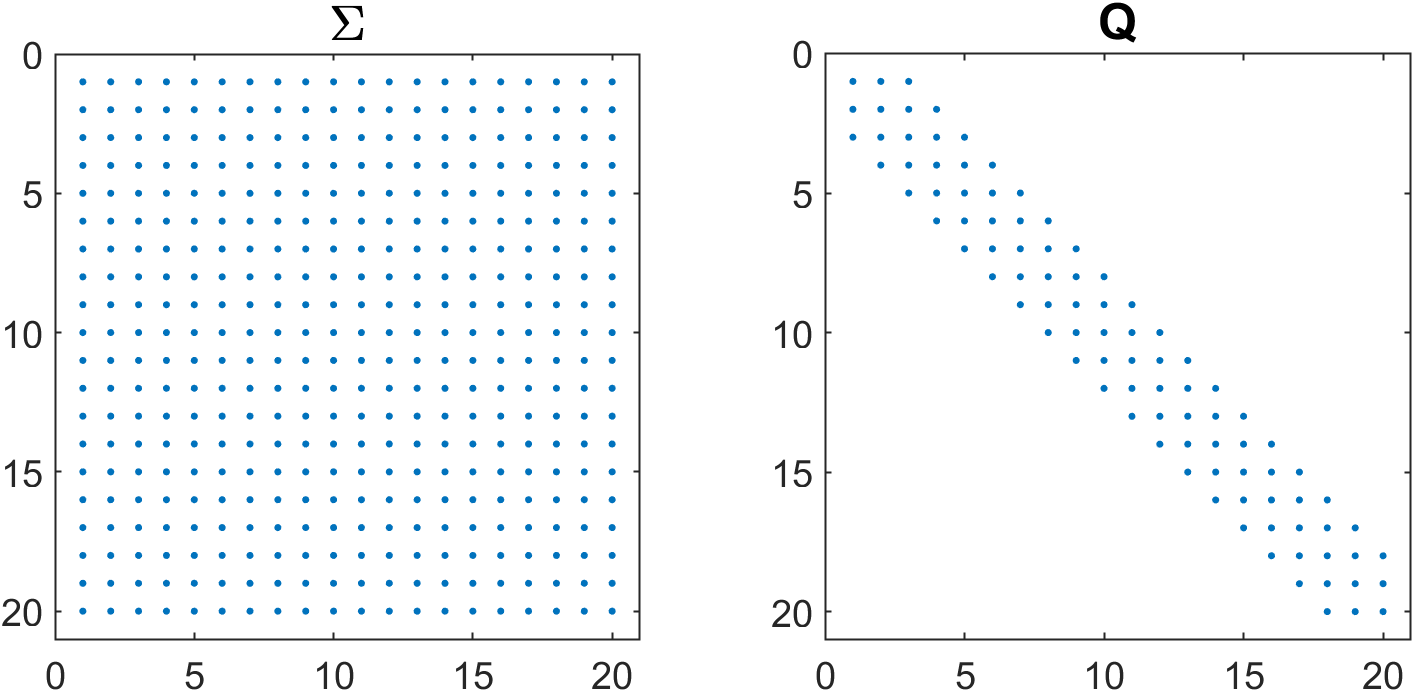
\includegraphics[scale = 0.65]{fig_Sigma_Q.png}  \vspace{0.1cm} \\
        \end{figure}
            \setstretch{0.1}
            {\tiny \textbf{Notes}: The blue dots indicate the non-zero entries in the covariance matrix $\Sigma$ and precision matrix $\mathbf{Q}$ of an AR(2) process for $T=20$ observations. The former is a dense matrix while the latter is sparse and banded with lower and upper bandwidth equal to 2.}\par
    \end{adjustbox}
\end{frame}

\begin{frame}[fragile]{Precision-based sampling}{Computational advantages of banded precision matrices}

    Solving linear systems of the form $Ux = b$ where $U$ is an $n \times n$ upper-triangular matrix takes $n^2$ flops (left); when U has bandwidth $p$ the solution can be obtained in $2 n p$ flops (right):

    \begin{columns}
        \column{0.5\textwidth}
        \begin{lstlisting}
    % solution to Ux = b
    % U has maximal bandwidth
    for i = n:-1:1
        x(i) = b(i)/U(i,i)
        for j = 1:i-1
            b(j) = b(j) - U(j,i)x(i)
        end
    end
        \end{lstlisting}
        %\hfill
        \column{0.5\textwidth}
        \begin{lstlisting}
% solution to Ux = b
% U has bandwidth p            
for i = n:-1:1
    x(i) = b(i)/U(i,i)
    for j = (*@\textcolor{red}{\,\textbf{max}\,\{1\,,\,i\,\textendash\,p\,\}}@*):i-1
        b(j) = b(j) - U(j,i)x(i)
    end
end
        \end{lstlisting}
    \end{columns}
    \vspace{0.3cm}

    Even larger gains for matrix factorisations, e.g. Cholesky ($Q = L\transpose{L}$) $\Longrightarrow$ linear instead of cubic costs! \\~\\

    $L$ "inherits" the bandwidth of $Q$ \citep[][Theorem 4.3.1]{golubvanloan2013}
\end{frame}

\begin{frame}{Precision-based sampling}{Factor model}
    To fix ideas, consider the following factor model:
    \begin{align*}
        \mathbf{y}_t &= \lambda \boldsymbol{\eta}_t + \mathbf{e}_t \\
        \mathbf{e}_t &= \phi^{e} \mathbf{e}_{t-1} + \boldsymbol{\epsilon}_t;\: \boldsymbol{\epsilon}_t \sim \mathcal{N}(0, diag([\sigma^2_1, \cdots, \sigma^2_N])) \\
        \boldsymbol{\eta}_t &= \phi^{\eta} \boldsymbol{\eta}_{t-1} + \mathbf{u}_t;\: \mathbf{u}_t \sim \mathcal{N}(0, \Sigma_u)
    \end{align*}

    where $\mathbf{y}_t$ is an $N\times 1$ vector of data and $\eta_t$ is an $R\times 1$ vector of unobserved factors \\~\\

    Bayesian estimation of the model is done via a Gibbs Sampler which sequentially draws from \vspace{0.2cm}
    \begin{itemize}
        \item the conditional distribution of factors given data and parameters: $p(\boldsymbol{\eta} | \mathbf{y}, \Theta)$ 
        \item the conditional distribution of parameters given data and factors:$p(\Theta | \boldsymbol{\eta}, \mathbf{y})$
    \end{itemize}

    %where $\Theta = [\lambda, \phi^e, \phi^{\eta}, \Sigma_u, \sigma_1^2, \cdots, \sigma_N^2]$

\end{frame}

\begin{frame}[fragile]{Precision-based sampling}{Drawing from $p(\boldsymbol{\eta} | \mathbf{y}, \Theta)$}
    \label{precsampl_draw_eta}
    Joint distribution of states $\boldsymbol{\eta} = \transpose{[\transpose{\boldsymbol{\eta}_1}, \cdots, \transpose{\boldsymbol{\eta}_T}]}$ and data $\mathbf{y} = \transpose{[\transpose{\mathbf{y}}_1, \cdots, \transpose{\mathbf{y}}_T]}$ given parameters: 
    $$
            \mathbf{z} =
            \begin{bmatrix}
                \boldsymbol{\eta} \\ 
                \mathbf{y}
            \end{bmatrix}     
            \sim        
            \mathcal{N}(\mathbf{0}, \mathbf{Q}^{-1})
            ; \: \mathbf{Q} = 
            \begin{bmatrix}
                \mathbf{Q}_{\eta} & \mathbf{Q}_{\eta y} \\
                \mathbf{Q}_{\eta y}' & \mathbf{Q}_{y}
            \end{bmatrix}   
            \hyperlink{app_mapping}{\beamerbutton{Mapping from $\Theta$ to $\mathbf{Q}$}} 
    $$ \\~\\    
    
    Standard result for the multivariate $\mathcal{N}$: $p(\boldsymbol{\eta} | \mathbf{y}, \Theta) = \mathcal{N}(-\mathbf{Q}_{\eta}^{-1} \mathbf{Q}_{\eta y} \mathbf{y}, \mathbf{Q}_{\eta}^{-1})$\\~\\

    Sampling from this distribution does \textbf{not} require the inversion of (the potentially very large matrix) $\mathbf{Q}_{\eta}$ and because it is banded, 
    \vspace{0.2cm}
    \begin{itemize}
        \item the mean $-\mathbf{Q}_{\eta}^{-1} \mathbf{Q}_{\eta y} \mathbf{y}$ 
        \item and a random draw given mean and precision matrix 
    \end{itemize}
    \vspace{0.2cm}
    can be obtained efficiently! \hyperlink{app_rueheld_algs}{\beamerbutton{\citet[][Algorithms 2.1, 2.4]{rueheld_book2005}}}
    
\end{frame}

\begin{frame}{Precision-based sampling with missing observations}{Drawing from $p(\boldsymbol{\eta}, \mathbf{y}^m | \mathbf{y}^o, \Theta)$}
    
\end{frame}

\begin{frame}[t, allowframebreaks]{References}
    \scriptsize     
    \bibliographystyle{aer}
    \bibliography{biblio}
\end{frame}

\begin{frame}{Appendix}{Mapping from $\Theta$ to $\mathbf{Q}$}
\label{app_mapping}
ladida
ladida
\end{frame}

\begin{frame}{Appendix}{\citet[][Algorithm 2.1, 2.4]{rueheld_book2005}}
    \label{app_rueheld_algs}
    \setcounter{algorithm}{0}
    \begin{algorithm}[H]
        \caption{Solving $\mathbf{A} \mathbf{x} = \mathbf{b}$ where $\mathbf{A} > 0$}
        \begin{algorithmic}[1]
            \State Compute the Cholesky factorization $\mathbf{A} = \mathbf{L}\transpose{\mathbf{L}}$
            \State Solve $\mathbf{L}\mathbf{v} = \mathbf{b}$ via forward substitution
            \State Solve $\transpose{\mathbf{L}}\mathbf{x} = \mathbf{v}$ via backward substitution\\
            \Return $\mathbf{x}$
        \end{algorithmic}
    \end{algorithm}
    \setcounter{algorithm}{3}
    \begin{algorithm}[H]
        \caption{Sampling $\mathbf{x} \sim \mathcal{N}(\boldsymbol{\mu}, \mathbf{Q}^{-1})$}
        \begin{algorithmic}[1]
            \State Compute the Cholesky factorization $\mathbf{Q} = \mathbf{L}\transpose{\mathbf{L}}$
            \State Sample $\mathbf{z} \sim \mathcal{N}(\boldsymbol{\mu}, \mathbf{I})$
            \State Solve $\transpose{\mathbf{L}} \mathbf{v} = \mathbf{z}$
            \State Compute $\mathbf{x} = \boldsymbol{\mu} + \mathbf{v}$\\
            \Return $\mathbf{x}$
        \end{algorithmic}
    \end{algorithm}

    \hyperlink{precsampl_draw_eta}{\beamerreturnbutton{Back}}
\end{frame}

\end{document}